 \begin{figure}[bt!]
  \begin{center}
    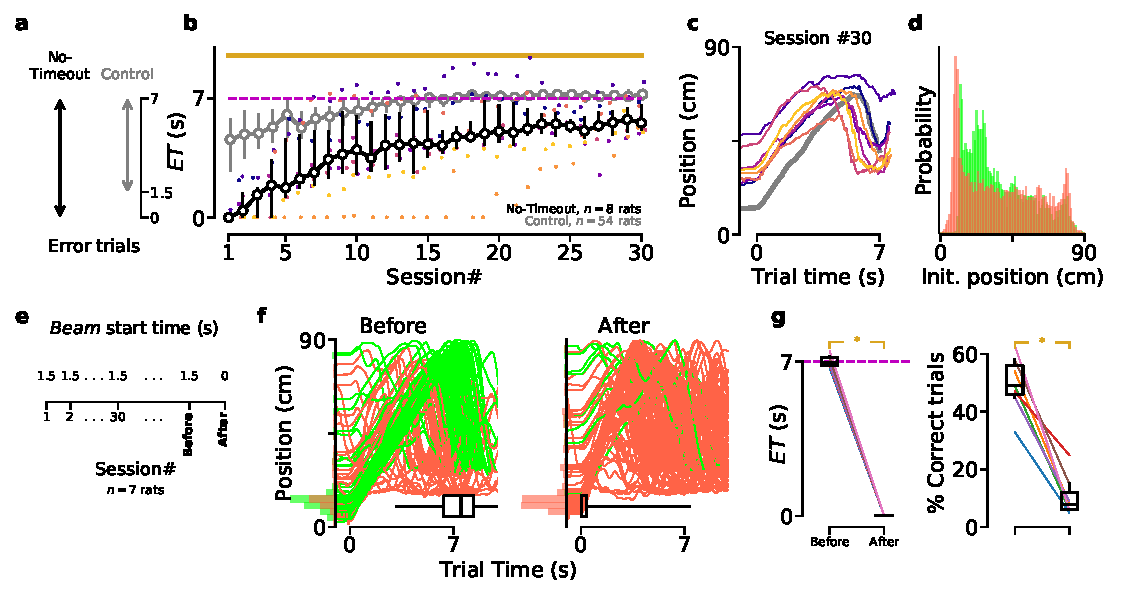
\includegraphics[scale=1]{ch-time/figures/NToTrd.pdf}
    \caption[No-Timeout Condition]
    {\textbf{Decreased temporal accuracy when animals are penalized for starting trials in the reward area.}
    \textbf{a)}
    In the control condition, animals had a 1.5~s timeout period to leave the reward area after motor onset.
    In ``no-timeout'' condition, crossing the infrared beam any time before 7~s registers as an error trial.
    \textbf{b)}
    Median $ET$ for animals trained in the no-timeout (black), and control (gray) conditions.
    Colored dots indicate performance for individual no-timeout animals.
    \textbf{c)}
    Median trajectory of no-timeout animals (same colors as in panel~b) in session~\#30.
    \textbf{d)}
    PDF of the no-timeout animals' positions at the beginning of each trial, from sessions~\#20 to~\#30.
    \textbf{e)}
    After extensive training in control condition, animals ($n=7$) were tested in a no-timeout probe session, in which the beam started at the beginning of the trial, rather than 1.5~s later.
    \textbf{f)}
    Trajectories of a representative animal in the last control session (\textit{left}), and the probe session (\textit{right}).
    \textbf{g)}
    Median $ET$s (\textit{left}), and percentage of correct trials (\textit{right}) in the sessions immediately before and after the change in beam start time.
    Each line represents a single animal.
    Asterisks indicate significant differences (non-parametric paired comparison, see \autoref{ch:methods:tech}).
    }
    \label{fig:time:ntoTrd}
  \end{center}
\end{figure}
